\documentclass{article}
\usepackage{hyperref}
\usepackage{amssymb, mathtools, amsmath}
\usepackage[dvipsnames]{xcolor}
\usepackage{graphicx}
\usepackage{float}
\usepackage{caption}
\usepackage{hyperref}
\hypersetup{
    colorlinks=true,
    linkcolor=blue,
    filecolor=magenta,      
    urlcolor=blue,
}

\title{ Macroeconomic Theory
        \thanks{Course instructed by Professor Christoph Hedtrich.} \\
        Homework 5: Real Business Cycle Models
        }

\author{
        % Add your name here
        Uppsala Masters in Economics 2021-2022
        }

\date{25 November 2021}

% margins
\oddsidemargin 3mm
\evensidemargin 3mm
\topmargin -12mm
\textheight 600pt
\textwidth 420pt

% no indent
\setlength\parindent{0pt}
% \renewcommand{\theenumi}{\thesection(\alph{enumi})}
% \renewcommand\thesubsection{\arabic{subsection}}

% custom commands
\newcommand{\E}[1]{\mathrm{E}\left[#1\right]}
\newcommand{\Et}[1]{\mathrm{E}_t\left[#1\right]}
\newcommand{\cov}[1]{\mathrm{Cov}\left(#1\right)}
\newcommand{\var}[1]{\mathrm{Var}\left(#1\right)}
\renewcommand{\L}{\mathcal{L}}

\begin{document}
    
    \maketitle
    \section{The RBC Model}
    
    \subsection{Production}
        
        Economy consists of large number of identical competitive (price-taking) firms, where total output $Y_t$ in period $t$ is Cobb-Douglas,
        \begin{align}
            Y_t &= K_t^\alpha \left( A_t L_t\right)^{1-\alpha}, \quad \alpha \in (0, 1),
            \\
            &= I_t + C_t + G_t
        \end{align}
        
        where $K_t$, $A_t$, $L_t$ are capital, technology, and labor. $Y_t$ is also divided among $I_t$, $C_t$, and $G_t$, which are investment, consumption, and government spending. \textbf{Capital} follows the law of motion
        \begin{align}
            K_{t+1} &= K_t - \delta K_{t} + I_t \\
            &= (1 - \delta) K_{t} + (Y_t - C_t - G_t)
        \end{align}
        
        where $\delta$ is the capital depreciation rate. \textbf{Technology} follows the law of motion
        \begin{align}
            \ln(A_t) &= \bar{A} + gt + \tilde{A}_t
            \\
            \implies
            A_t
            &= e^{\bar{A} + \tilde{A}_t}e^{gt},
            \quad \frac{\dot{A}_t}{A_t}
            = g + \frac{\dot{\tilde{A}}_t}{\tilde{A}_t},
        \end{align}
        where $\tilde{A}_t$ is a ``technology shock" with a AR(1) process
        \begin{align}
            \tilde{A}_{t} = \rho_A \tilde{A}_{t-1} + \epsilon_{A, t},
            \quad \rho_A \in (-1, 1),
            \quad \E{\epsilon_{A, t}} = 0.
        \end{align}
        
        and $\epsilon_{A, t}$ are independently and identically distributed (i.i.d.) across periods. \textbf{Government spending} is financed by lump-sum taxes on production that equal to spending each period (so taxes do not impact model\footnote{Tax rate $\tau_t$ in period $t$ and $G_t = T_t$, then after tax $Y_t - T_t = C_t + I_t + G_t - T_t = C_t + I_t$.}), and follows the law of motion
        \begin{align}
            \ln(G_t) &= \bar{G} + (n + g)t + \tilde{G}_t,
            \\
            \tilde{G}_t &= \rho_G \tilde{G}_{t - 1} + \epsilon_{G, t},
            \quad \rho_G \in (-1, 1),
        \end{align}
        and $\E{\epsilon_{G, t}} = 0$ and are i.i.d. across time.
        
        Perfectly competitive firms maximize profits in each period, $\Pi_t = Y_{t} - w_t L_t - (r_t + \delta_t) K_t$. First order conditions imply factor costs are equal to marginal products,
        \begin{align}
            w_t &= \frac{\partial Y_t}{\partial L_t} = (1-\alpha) \left(\frac{K_t}{A_t L_t}\right)^\alpha,
            \label{eqn:wage}
            \\
            r_t &= \frac{\partial Y_t}{\partial K_t} = \alpha \left(\frac{A_t L_t}{K_t}\right)^{1-\alpha}.
            \label{eqn:interest}
        \end{align}
        
    \subsection{Households}
        
        Let $N_t$ be the population in the economy in a period over $H$ identical households. Member per household is given by $N_t / H$, and population grows exogenously at a constant continuous rate:
        \begin{align}
            \ln N_t &= \bar{N} + nt \\
            \implies
            N_t &= e^{\bar{N}}e^{nt}. \label{eqn:population}
        \end{align}
        
        Per capita consumption and labor is
        \begin{align}
            c_t &= \frac{C_t}{N_t}, \quad
            \ell_t = \frac{L_t}{N_t} \in [0, 1]
        \end{align}
        
        Labor $\ell_t$ is normalized to percentage of time endowment, and leisure per capita is defined as $1-\ell_t$. In any period $t$, the representative individual's utility is given by
        \begin{align}
            u_t(c_t, \ell_t) = \ln c_t + b \ln(1-\ell_t),
            \quad b > 0,
        \end{align}
        
        where each period is discounted by the parameter $\rho > n$. Putting it all together, the \textbf{representative household} (with $N_t/H$ members) maximizes expected utility
        \begin{align}
            U &= \sum_{t=0}^\infty e^{-\rho t}
            \bigg( \ln c_t + b \ln(1-\ell_t) \bigg)
            \frac{N_t}{H}
            \\
            \quad s.t. &\quad
            \sum_{t=0}^{\infty}
            \frac{c_t}{\prod_{s=1}^{t}(1+r_s)} \frac{N_t}{H}\le
            \sum_{t=0}^{\infty}
            \frac{w_t \ell_t}{\prod_{s=1}^{t}(1+r_s)} \frac{N_t}{H}.
        \end{align}
        
        Form the Lagrangian
        \begin{align}
            \L
            = \sum_{t=0}^\infty e^{-\rho t}
            \bigg( \ln c_t + b \ln(1-\ell_t) \bigg)
            \frac{N_t}{H} 
            + \lambda \left(
                \sum_{t=0}^{\infty}
                \frac{w_t \ell_t - c_t}{\prod_{s=1}^{t}(1+r_s)}\frac{N_t}{H}
                \right)
        \end{align}
        
        and we have the following FOC for each period $t$ that
        \begin{align}
            \frac{\partial \L}{\partial c_t} = 0
            &\implies
            \frac{1}{c_t}\frac{N_t}{H}e^{-\rho t}
            = \frac{\lambda}{\prod_{s=1}^{t}(1+r_s)} \frac{N_t}{H}, 
            \label{eqn:foc-1}
            \\
            \frac{\partial \L}{\partial \ell_t} = 0
            &\implies
            \frac{b}{1 - \ell_t}\frac{N_t}{H}e^{-\rho t}
            = \frac{\lambda w_t}{\prod_{s=1}^{t}(1+r_s)}\frac{N_t}{H}.
            \label{eqn:foc-2}
        \end{align}
        
        
        Combining the above for two periods $t$ and $t+1$, we have the Euler equations:
        \begin{align}
            \frac{c_t}{c_{t+1}}
            &= \frac{e^{\rho}}{1+r_{t+1}},
            \label{eqn:euler-c}
            \\
            \frac{1-\ell_t}{1-\ell_{t+1}}
            &= \frac{e^{\rho}}{1+r_{t+1}}\frac{w_{t+1}}{w_t}
            \label{eqn:euler-ell}
        \end{align}
        See Appendix~\ref{app:euler-c-ell} for details of derivations. Suppose that
        
    \subsection{Uncertainty}
    
        By  \eqref{eqn:wage} and \eqref{eqn:interest}, future equilibrium wages $w_t$ and interest rates $r_t$ are uncertain, as they depend on $A_t$ which has a stochastic component. At period $t$,
        the expected utility continuation utility is
        \begin{align}
            U_t &= \Et{\sum_{s=0}^\infty e^{-\rho (t+s)}
            \bigg( \ln c_{t+s} + b \ln(1-\ell_{t+s}) \bigg)
            \frac{N_t}{H}}
            \label{eqn:stoch-utility}
            % \\
            % &= \sum_{s=0}^\infty \left(
            %     \Et{\ln c_{t+s}} + \Et{b \ln(1-\ell_{t+s})}
            % \right)
            % \frac{N_t}{H}e^{-\rho (t+s)}
            \\ s.t. \quad
             & \Et{\sum_{t=0}^{\infty}
             \frac{c_{t+s}}{\prod_{\tau=1}^{{t+1}}(1+r_\tau)}
             \frac{N_t}{H}} \le
            \Et{\sum_{t=0}^{\infty}
            \frac{w_{t+s} \ell_{t+s}}{\prod_{\tau=1}^{{t+1}}(1+r_\tau)}
            \frac{N_t}{H}}.
            \label{eqn:stoch-bc}
        \end{align}
        
        Consider consumption budget of two consecutive periods $t$ and $t+1$. By \eqref{eqn:stoch-bc}, the household consumption budget is
        \begin{align}
            c_{t}\frac{N_{t}}{H} + \Et{\frac{c_{t+1}}{1+r_{t+1}}\frac{N_{t+1}}{H}}
            &= (c_{t} - \Delta c)\frac{N_{t}}{H}
            + \Et{\frac{(c_{t+1} + (1+r_{t+1})e^{-n}\Delta c)}{(1+r_{t+1})} \frac{N_{t+1}}{H}}
            \label{eqn:bc-delta-c}
        \end{align}
        
        Thus, a change of $-\Delta c$ in  $c_t$ should result in a change of $(1+r_{t+1}) e^{-n} \Delta c$ in $c_{t+1}$ within the budget constraint. See Appendix \ref{app:bc-delta-c} for details of the derivation. \\
        
        On the optimal path, allowing changes in $c_t$ and $c_{t+1}$ within the budget constraint, we have the ``stochastic'' Euler equation:
        \begin{align}
            \frac{1}{c_t}
            &= e^{-\rho} \Et{\frac{1+r_{t+1}}{c_{t+1}}}
            \label{eqn:euler-c-stoch}
        \end{align}
        See Appendix \eqref{app:euler-c-stoch} for details.
        
    
    \section{Question 1: DR 5.7.}
        
        \begin{figure}[H]
            \centering
            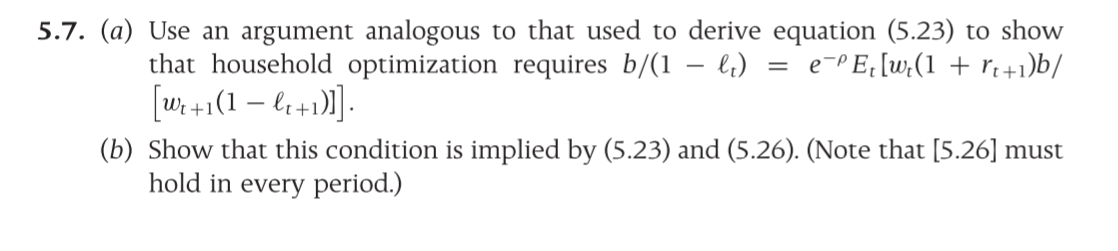
\includegraphics[width=\textwidth]{./HW5-DR5.7.png}
        \end{figure}
        
        
        \begin{itemize}
            \item[(a)]
            Total household income from labor wages is given by
            \begin{align}
                & w_t \ell_t \frac{N_t}{H}
                + \Et{ \frac{w_{t+1} \ell_{t+1}}{(1+r_{t+1})} \frac{N_{t+1}}{H} }
                \\
                =& \left(
                    w_t \ell_t \frac{N_t}{H} - w_t \Delta \ell \frac{N_t}{H}
                \right)
                + \Et{\frac{w_{t+1} \ell_{t+1}}{(1+r_{t+1})} \frac{N_{t+1}}{H} } + w_t \Delta \ell \frac{N_t}{H}
                \\
                =& w_t (\ell_t - \Delta \ell)\frac{N_t}{H} + \Et{\frac{w_{t+1} \ell_{t+1}N_{t+1} + (1+r_{t+1}) w_t N_{t} \Delta \ell}{(1+r_{t+1})H}}
                \\
                =& w_t (\ell_t - \Delta \ell) + \Et{\frac{w_{t+1} N_{t+1} \left(\ell_{t+1} +  (1+r_{t+1}) \frac{w_t}{w_{t+1}} \frac{N_t}{N_{t+1}} \Delta \ell \right)}{(1+r_{t+1})H}}
                \\
                =& w_t (\ell_t - \Delta \ell) + \Et{\frac{w_{t+1} \left(\ell_{t+1} + (1+r_{t+1})e^{-n} \frac{w_t}{w_{t+1}} \Delta \ell \right)}{(1+r_{t+1})} \frac{N_{t+1}}{H} },
            \end{align}
        
        thus a change in labor $-\Delta \ell$ in $\ell_t$ results in a change in labor of $(1+r_{t+1})e^{-n}\frac{w_t}{w_{t+1}} \Delta \ell$ in $\ell_{t+1}$. Then on the optimal path
        \begin{align}
            dU_t = 0
            &= \frac{\partial U_t}{\partial \ell_t} d \ell_t
            + \frac{\partial U_t}{\partial \ell_{t+1}} d \ell_{t+1}
            \\
            &= -\frac{b}{1 - \ell_t}\frac{N_t}{H}e^{-\rho t} d \ell_t
            -\Et{\frac{b}{1 - \ell_{t+1}}\frac{N_{t+1}}{H}e^{-\rho (t+1)} d \ell_{t+1}}
            \\
            &= -\frac{b}{1 - \ell_t}\frac{N_t}{H}e^{-\rho t} \Delta \ell
            + \Et{\frac{w_t b (1+r_{t+1})}{w_{t+1}(1 - \ell_{t+1})}\frac{N_{t+1}}{H}e^{-\rho (t+1)}e^{-n} \Delta \ell}
            \\
            \implies
            \frac{b}{1 - \ell_t}\frac{N_t}{H}e^{-\rho t} \Delta \ell
            &= \Et{\frac{w_t b (1+r_{t+1})}{w_{t+1} (1 - \ell_{t+1})}}\frac{N_{t+1}}{H}e^{-\rho (t+1)}e^{-n} \Delta \ell
            \\
            \implies
            \frac{b}{1 - \ell_t}
            &= \frac{N_{t+1}}{N_t} e^{-n} e^{-\rho} \Et{\frac{w_t b (1+r_{t+1})}{w_{t+1}(1-\ell_{t+1})}}
            \\
            &= e^{-\rho} \frac{w_t b}{w_{t+1}}\Et{\frac{1+r_{t+1}}{1 - \ell_{t+1}}}.
        \end{align}
        
        \item[(b)]
        
        In any period, the one period budget constraint is $\Delta c = w_t \Delta \ell$, then at the optimal single-period choice we have
        \begin{align}
            d u = 0
            = \frac{\partial u}{\partial c_t} d c_t + \frac{\partial u}{\partial \ell_t} d \ell_t
            &= \frac{1}{c_t} dc_t
            - \frac{b}{1 - \ell_t} d\ell_t
            \\
            \implies 0 &= \frac{1}{c_t} w_t \Delta \ell
            - \frac{b}{1 - \ell_t} \Delta \ell
            \\
            \implies
            \frac{1}{c_t} w_t \Delta \ell
            &= \frac{b}{1 - \ell_t} \Delta \ell
            \\
            \implies
            \frac{1}{c_t}
            &= \frac{b}{w_t(1 - \ell_t)}.
        \end{align}
        
        Which gives us a relationship for the optimal within-period consumption and labor choice. Then with optimal intertemporal consumption choice in \eqref{eqn:euler-c-stoch}, we have that
        \begin{align}
            \frac{1}{c_t}
            &= e^{-\rho} \Et{\frac{1+r_{t+1}}{c_{t+1}}}
            \\ \implies
            \frac{b}{w_t(1 - \ell_t)}
            &= e^{-\rho} \Et{\frac{(1+r_{t+1})b}{w_{t+1} (1-\ell_{t+1})}}
            \\ \implies
            \frac{b}{(1 - \ell_t)}
            &= e^{-\rho} \frac{w_t b}{w_{t+1}}\Et{\frac{1+r_{t+1}}{1-\ell_{t+1}}}
        \end{align}
        
        \end{itemize}
    

    \appendix
    \section{Appendix: Derivations}
    
    \subsection{Derivations for (\ref{eqn:euler-c}) and (\ref{eqn:euler-ell})}\label{app:euler-c-ell}
        
        By FOCs \eqref{eqn:foc-1} and \eqref{eqn:foc-2},
        \begin{align}
            \frac{c_t}{c_{t+1}}
            &= \frac{e^{-\rho t}
                \left[\prod_{s=1}^{t}(1+r_s)\right] / \lambda}
                {e^{-\rho (t+1)} \left[\prod_{s=1}^{t+1}(1+r_s)\right] / \lambda}
            \\
            &= \frac{e^{\rho}}{1+r_{t+1}}
            \\
            \frac{1-\ell_t}{1-\ell_{t+1}}
            &= \frac{- b e^{-\rho t}
                    \left[\prod_{s=1}^{t}(1+r_s)\right] / (\lambda w_t)}
                    {- b e^{-\rho (t+1)}
                    \left[\prod_{s=1}^{t+1}(1+r_s)\right] / (\lambda w_{t+1})}
            \\
            &= \frac{e^{\rho}}{1+r_{t+1}}\frac{w_{t+1}}{w_t}
        \end{align}
    
    \subsection{Derivation for (\ref{eqn:bc-delta-c})}\label{app:bc-delta-c}
        Note that $\frac{N_t}{N_{t+1}} = e^{-n}$ by \eqref{eqn:population}. At period $t$, the present value of  consumption in periods $t$ and $t+1$ is
        \begin{align}
            c_{t}\frac{N_{t}}{H} + \Et{\frac{c_{t+1}}{1+r_{t+1}}\frac{N_{t+1}}{H}}
            &= \left(c_{t}\frac{N_{t}}{H} - \Delta c \frac{N_{t}}{H} \right)+ \Et{ \frac{c_{t+1}N_{t+1}}{(1+r_{t+1})H}} + \Delta c \frac{N_{t}}{H}
            \\
            &= (c_{t} - \Delta c)\frac{N_{t}}{H}
            + \Et{ \frac{c_{t+1}N_{t+1}}{(1+r_{t+1})H}+ \Delta c \frac{N_{t}}{H} }
            \\
            &= (c_{t} - \Delta c)\frac{N_{t}}{H}
            + \Et{\frac{c_{t+1} N_{t+1} + (1+r_{t+1}) \Delta c N_t}{(1+r_{t+1})H}}
            \\
            &= (c_{t} - \Delta c)\frac{N_{t}}{H}
            + \Et{\frac{\left( c_{t+1}
                + (1+r_{t+1}) \frac{N_t}{N_{t+1}} \Delta c \right)}{(1+r_{t+1})}\frac{N_{t+1}}{H}}
            \\
            &= (c_{t} - \Delta c)\frac{N_{t}}{H}
            + \Et{\frac{\left( c_{t+1}
                + (1+r_{t+1}) e^{-n} \Delta c \right)}{(1+r_{t+1})}\frac{N_{t+1}}{H}}
        \end{align}
    
    \subsection{Derivation for (\ref{eqn:euler-c-stoch})}\label{app:euler-c-stoch}
    
    By \eqref{eqn:bc-delta-c}, a change of $-\Delta c$ in  $c_t$ results in a change of $(1+r_{t+1}) e^{-n} \Delta c$ in $c_{t+1}$ within the budget constraint. On the optimal path, utility remains constant with a slight shift in $c_{t}$ within the budget constraint. Then we have that
    \begin{align}
            d U_t = 0
            &= \frac{\partial U_t}{\partial c_t} dc_t + \frac{\partial U_t}{\partial c_{t+1}} dc_{t+1}
            \\
            &= \frac{1}{c_t}\frac{N_t}{H}e^{-\rho t} dc_t + \Et{\frac{1}{c_{t+1}}\frac{N_{t+1}}{H}e^{-\rho (t+1)} dc_{t+1}}
            \\
            &= \frac{1}{c_t}\frac{N_t}{H}e^{-\rho t} \Delta c + \Et{\frac{1}{c_{t+1}}\frac{N_{t+1}}{H}e^{-\rho (t+1)}  (-(1+r_{t+1})e^{-n}  \Delta c)}
            \\ \implies
            \frac{1}{c_t} \frac{N_t}{H}e^{-\rho t} \Delta c
            &= \Et{\frac{1+r_{t+1}}{c_{t+1}}} \frac{N_{t+1}}{H}e^{-\rho (t+1)}e^{-n} \Delta c 
            \\ \implies
            \frac{1}{c_t}
            &= \Et{\frac{1+r_{t+1}}{c_{t+1}}} \frac{N_{t+1}}{N_t}e^{-n}e^{-\rho} = \Et{\frac{1+r_{t+1}}{c_{t+1}}} e^{-\rho}.
        \end{align}
    
\end{document}